\begin{ledgroupsized}[r]{120mm}
\footnotesize 
\count\Bfootins=1000
\pstart                
\noindent\textbf{\"{U}berlieferung:}   
\pend
\end{ledgroupsized}
\begin{ledgroupsized}[r]{114mm}
\footnotesize 
\pstart 
\parindent -6mm
\makebox[6mm][l]{\textit{L}}Konzept: LH XXXVII 5 Bl. 12. 1 Bl. 4\textsuperscript{o}. 25 Z. in der unteren H\"{a}lfte von Bl.~12~v\textsuperscript{o}, unmittelbar nach dem St\"{u}ck N. 31\textsubscript{2}.  \\Cc 2, Nr. 946
\pend
\end{ledgroupsized}
\vspace*{8mm}
\count\Bfootins=1200
\pstart%
\noindent%
[12~v\textsuperscript{o}]%
\pend%
\pstart%
\centering%
\noindent%
De\textso{ Detrimento Motus }
contemplatio Geometrica:\\
quod mirabili naturae ingenio repraesentat \textso{Logarithmos.}
\pend%
\vspace*{0.5em}%
\pstart%
\centering%
\noindent%
Dissertation Geometrique, DU FROTTEMENT\\%
\edtext{avec la}{\lemma{avec}\Bfootnote{\textit{(1)}\ un \textit{(2)}\ la \textit{L}}} decouuerte d'une propriet\'{e} admirable de la nature\\%
s\c{c}avoir:\edlabel{037,05_012v_z1}%
\edtext{}{{\xxref{037,05_012v_z1}{037,05_012v_z2}}\lemma{s\c{c}avoir:}\Bfootnote{\textit{(1)}\ que la perte de la force par le frottement represente les logarithmes \textit{(2)}\ que les forces residues  \textit{(a)}\ sont \textit{(b)}\ estant comme les nombres, les espaces parcourus  \textit{(aa)}\ dans un medium \textit{(bb)}\ avec une vistesse egale   \textbar\ except\'{e} qu'elle a est\'{e} diminu\'{e}e \textit{erg.}\ \textbar\  dans un medium   \textbar\ homogene \textit{erg.}\ \textbar\  qui resiste au mouuement; seront comme les logarithmes. \textit{(3)}\ que [...] parcourus  \textbar\ uniformement \textit{erg.}\ \textbar\ est [...] logarithmes. \textit{L}}}
que le rapport de la perte de la force aux espaces parcourus uniformement\\%
est celuy des nombres aux
\edlabel{037,05_012v_z3}%
\edtext{}{{\xxref{037,05_012v_z3}{037,05_012v_z4}}\lemma{logarithmes.}\Bfootnote{\textit{(1)}\ Si nous posons un corps meu  \textit{(a)}\ uniformement dans \textit{(b)}\ dans un Medium hom \textit{(c)}\ et dont la vistesse n'est  \textit{(aa)}\ diminu\'{e}e \textit{(bb)}\ alter\'{e}e que par le Medium homogene  \textit{(aaa)}\ dans lequel \textit{(bbb)}\ qui resiste \`{a} son mouuement \textit{(2)}\  Si nous posons un corps meu \textit{(3)}\ Car [...] homogene  \textbar\ $AC$ \textit{ erg.}\ \textbar\ , [...] et que \textit{(a)}\ la vistesse n'est \textit{(b)}\ sa premiere [...] resistance: \textit{L}}}%
logarithmes.%
\edlabel{037,05_012v_z2}%
\pend%
\vspace{1em}
\pstart
\noindent%
Car si nous posons qu'un corps $\displaystyle\bigcirc$ soit meu dans un medium homogene $AC,$ qui resiste \`{a} son mouuement;
et que sa premiere vistesse ne soit alter\'{e}e que par cette resistance\edlabel{037,05_012v_z4}:
%\pstart 
%\centering
%\noindent De\edtext{\textso{ Detrimento Motus }}{\lemma{}\Bfootnote{Detrimento Motus \ \textit{doppelt unterstrichen \ L}}}contemplatio Geometrica:\\
%quod mirabili naturae ingenio repraesentat \textso{Logarithmos}.
%\pend
%\pstart
%\centering
%Dissertation Geometrique, DU FROTTEMENT
%   \edtext{avec la}{\lemma{avec}\Bfootnote{\textit{(1)}\ un \textit{(2)}\ la \textit{L}}} decouuerte d'une propriet\'{e} admirable de la nature \edtext{s\c{c}avoir:
%   que le rapport de la perte de la force aux espaces parcourus uniformement est celuy des nombres aux logarithmes.}
%{\lemma{s\c{c}avoir:}\Bfootnote{\textit{(1)}\ que la perte de la force par le frottement represente les logarithmes \textit{(2)}\ que les forces residues  \textit{(a)}\ sont \textit{(b)}\ estant comme les nombres, les espaces parcourus  \textit{(aa)}\ dans un medium \textit{(bb)}\ avec une vistesse egale   \textbar\ except\'{e} qu'elle a est\'{e} diminu\'{e}e \textit{erg.}\ \textbar\  dans un medium   \textbar\ homogene \textit{erg.}\ \textbar\  qui resiste au mouuement; seront comme les logarithmes. \textit{(3)}\ que [...] parcourus  \textbar\ uniformement \textit{erg.}\ \textbar\ est [...] logarithmes. \textit{L}}}
%\pend
%\vspace{0,5em}
%\pstart
% \noindent Car si nous  \edtext{posons qu'un corps $\displaystyle\bigcirc$ soit meu dans un medium homogene $AC$, qui resiste \`{a} son mouuement; et que sa premiere vistesse ne soit alter\'{e}e que par cette resistance:}{\lemma{logarithmes.}\Bfootnote{\textit{(1)}\ Si nous posons un corps meu  \textit{(a)}\ uniformement dans \textit{(b)}\ dans un Medium hom \textit{(c)}\ et dont la vistesse n'est  \textit{(aa)}\ diminu\'{e}e \textit{(bb)}\ alter\'{e}e que par le Medium homogene  \textit{(aaa)}\ dans lequel \textit{(bbb)}\ qui resiste \`{a} son mouuement \textit{(2)}\  Si nous posons un corps meu \textit{(3)}\ Car [...] homogene  \textbar\ $AC$ \textit{ erg.}\ \textbar\ , [...] et que \textit{(a)}\ la vistesse n'est \textit{(b)}\ sa premiere [...] resistance: \textit{L}}} 
   alors les forces residues (:~par exemple celle, qui reste au \edtext{corps $\displaystyle\bigcirc$ quand il est arriv\'{e} \`{a} l'endroit $B$, ou $C$~:\phantom(\hspace{-1.2mm}) decroissant comme les nombres, (\hspace{-1.2mm}\phantom): au dessous de l'unit\'{e}}{\lemma{corps $\displaystyle\bigcirc$}\Bfootnote{\textit{(1)}\ en $B$   \textbar\ au dessous de l'u \textit{ erg.}\ \textbar\  \textit{(2)}\ quand [...] ou $C$~:\phantom(\hspace{-1.2mm}) \textit{(a)}\ seront \textit{(b)}\ estant \textit{(c)}\ decroissant [...] nombres, \textit{(aa)}\ (par exemple comme 1 \`{a} 2)  \textit{(aaa)}\ leur \textit{(bbb)}\ les espaces \textit{(bb)}\ (\hspace{-1.2mm}\phantom): au [...] l'unit\'{e} \textit{L}}} comme 1. $\rule[-4mm]{0mm}{10mm}\displaystyle\frac{1}{4}$ 
   %\pageparbreak
   ou de la progression decroissante au lieu qu'elle croist dans les tables des logarithmes~:) les espaces $AB$, $AC$ croistront comme les logarithmes.
   \pend
   \pstart
Non est opus Tabulas continuari progressione Geometrica decrescente, possumus enim uti jam calculatis altius incipiendo, v.g. non ab 1. sed ab 100, et inde decrescendo versus 1. Ex Tabulis Logarithmorum eligamus numeros, quia circiter integris et brevibus numeris exhiberi possunt, et experimentis, pilae in plano polito provolutae, vel cylindri in tabula betulina propulsi, vel naviculae in aqua progredientis, videatur an circiter consentiant experimento.
\pend
\count\Bfootins=1500
\vspace{1.5em}
\pstart
%\begin{wrapfigure}[14]{l}{0.13\textwidth}
%\vspace*{8mm}
%\begin{center}
    \noindent \centering 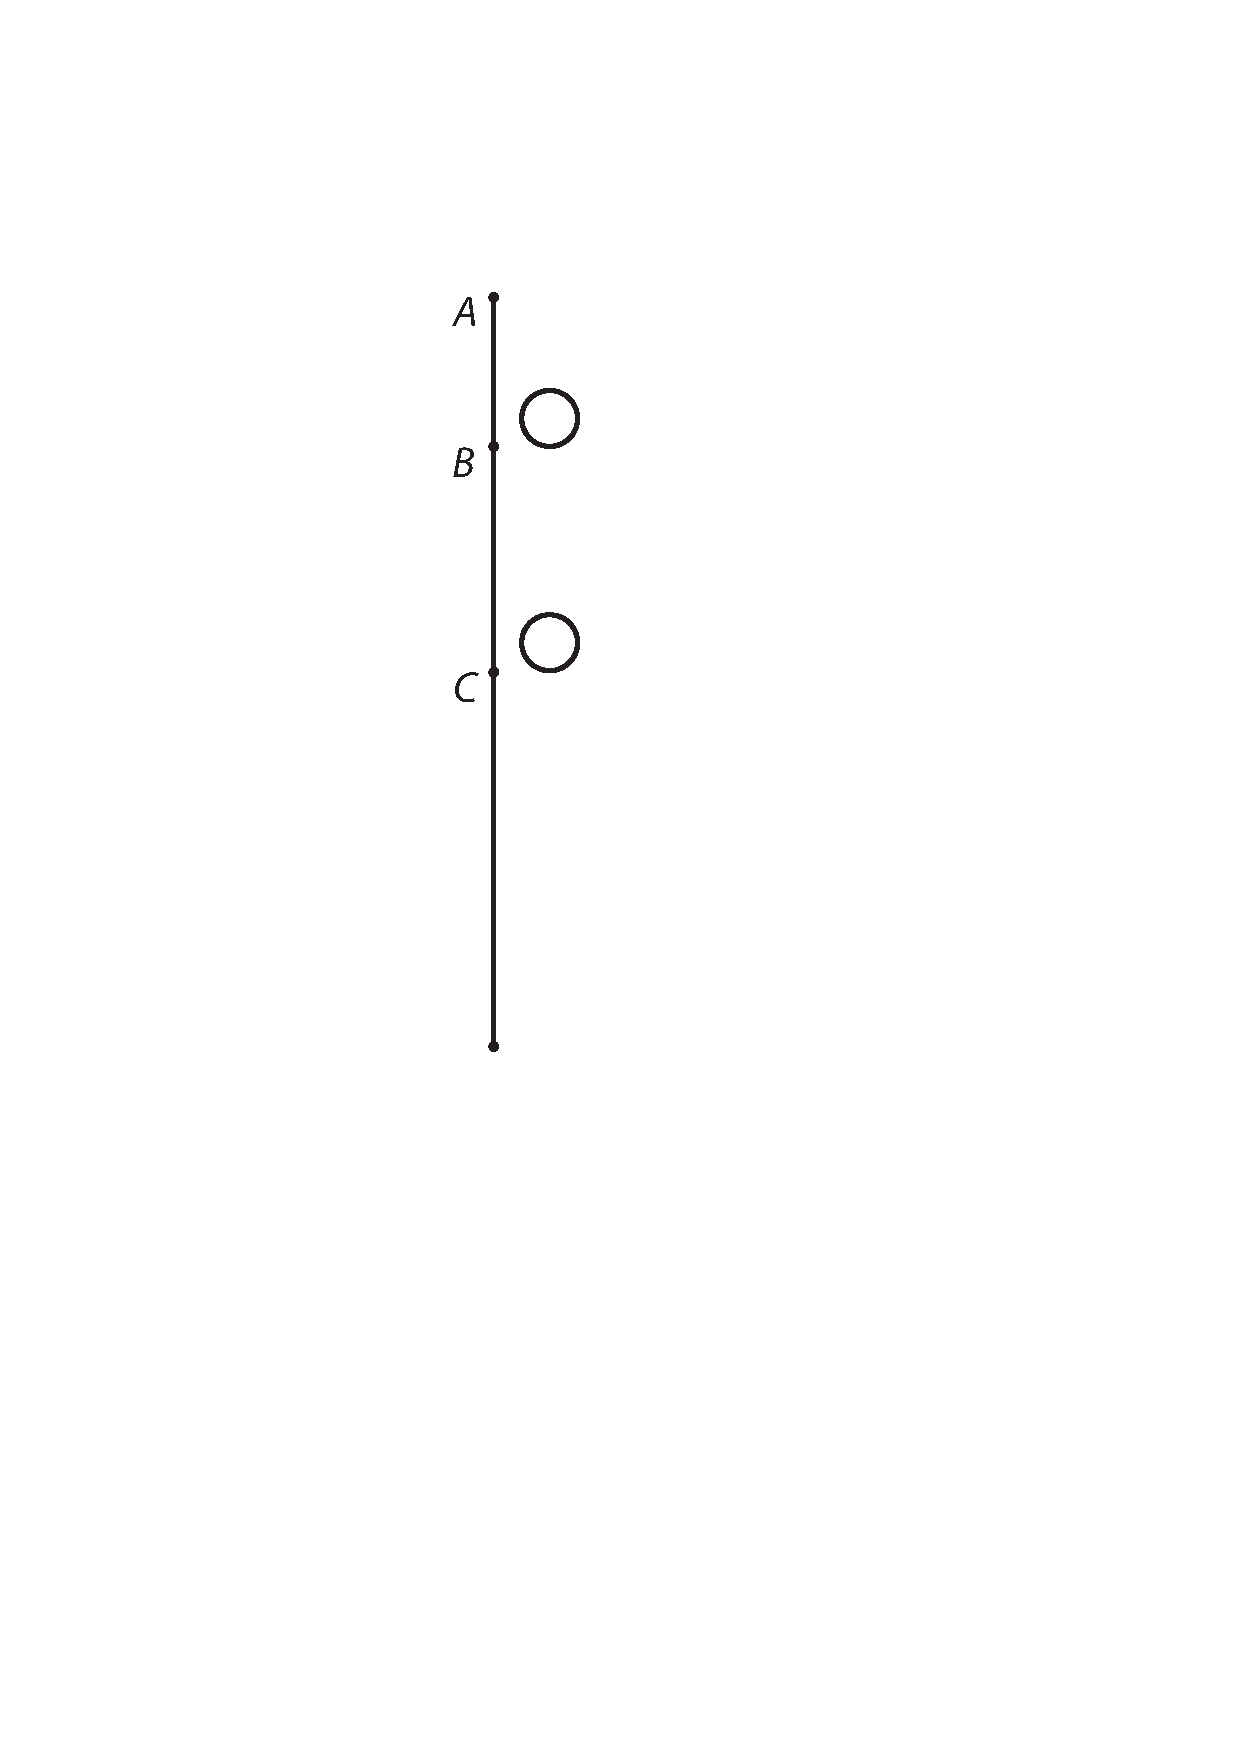
\includegraphics[trim = 0mm -3mm 0mm 0mm, clip, width=0.1\textwidth]{images/lh03705_012v_2-d1.pdf}\\
     \noindent \centering [\textit{Fig. 1}]  \setline{11}% \caption{Bildbeschreibung}
   % \end{wrapfigure}
   %\end{center}
    \pend